\documentclass[12pt,a4paper]{article}

\usepackage{graphicx}

\DeclareGraphicsExtensions{.pdf,.png,.jpg}

\begin{document}

\begin{center}

\begin{figure}
    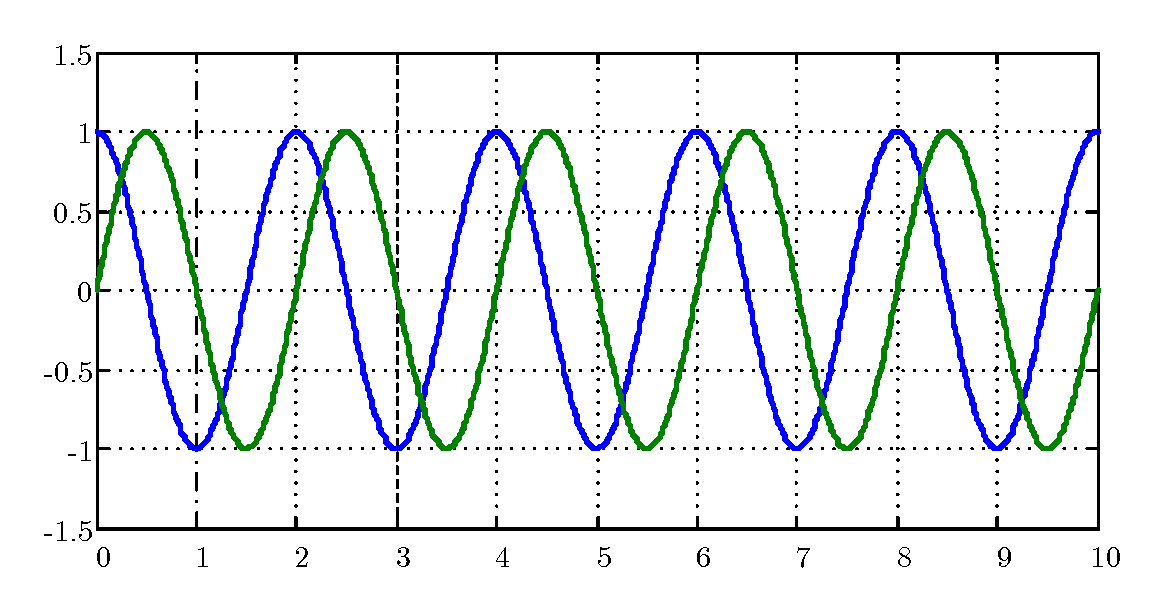
\includegraphics[scale=0.7]{Figs/Drawing1.pdf}
    \caption{My first plot exported from MATLAB\copyright}
    \label{fig.sine}
\end{figure}

\end{center}

The plots are given in Fig. \ref{fig.sine}. And first table is listed as Table \ref{table.first}.



\begin{center}

\begin{table}[b]
  \caption{Our first table}
  \label{table.first}
  \centering
  \begin{tabular}{|l|c||r|}
  \hline
  % after \\: \hline or \cline{col1-col2} \cline{col3-col4} ...
  One & Two & Three \\
  \cline{1-1}
  Four & Five & Six \\
  \cline{3-3}
  Seven & Eight & Nine \\
  \hline
  \end{tabular}
\end{table}


\end{center}




\end{document}